% Created 2014-04-14 一 20:23
\documentclass[10pt,b5paper]{article}
\usepackage{graphicx}
\usepackage{xcolor}
\usepackage{xeCJK}
\usepackage{longtable}
\usepackage{float}
\usepackage{textcomp}
\usepackage{geometry}
\geometry{left=0cm,right=0cm,top=0cm,bottom=0cm}
\usepackage{multirow}
\usepackage{multicol}
\usepackage{listings}
\usepackage{algorithm}
\usepackage{algorithmic}
\usepackage{latexsym}
\usepackage{natbib}
\usepackage{fancyhdr}
\usepackage[xetex,colorlinks=true,CJKbookmarks=true,linkcolor=blue,urlcolor=blue,menucolor=blue]{hyperref}


\usepackage{CJKutf8}
\begin{CJK}{UTF8}{gbsn}
\lstset{language=c++,numbers=left,numberstyle=\tiny,basicstyle=\ttfamily\small,tabsize=4,frame=none,escapeinside=``,extendedchars=false,keywordstyle=\color{blue!70},commentstyle=\color{red!55!green!55!blue!55!},rulesepcolor=\color{red!20!green!20!blue!20!}}
\author{Heyan Huang}
\date{\today}
\title{CS572 Project 3 Report}
\hypersetup{
  pdfkeywords={},
  pdfsubject={},
  pdfcreator={Emacs 24.3.50.1 (Org mode 8.2.5h)}}
\begin{document}

\maketitle
\tableofcontents

\begin{abstract}
In this project, I have implemented an genetic programming algorithm for the Sante Fe trail problem. By including the prog2, prog3 and isFoodAhead non-terminals, and left, right, and forward terminals, with completely no control of the tree generation except initial depth, the implementation creates an static ant, and the ant is able to evolve and behave evolutionarily and becomes smarter to pick up more and more food. The algorithm works with potential that by modifing and enforcing isFoodAhead non-terminal's forward node, or even an isFood2StepsAhead non-terminal, the algorithm could even work better or perfectly. In one work, the algorithm works great.
\end{abstract}

\begin{center}
\begin{tabular}{ll}
\hline
algorithms & Steady-state\\
\hline
Population Size & 100\\
Selection Method & Tournament Selection of size 10 each generation\\
Elitism(if used) & Yes, one copy of parent\\
Crossover Method & One-point Subtree crossover\\
Crossover rate & 1, happened 90\% on Non-terminal \& 10\% on Terminal\\
Mutation Method & Node mutation with probability of 0.45 at each node for the individual\\
Operator/non-terminal Set & add, subtract, multiply, divide, mypow, mysin, mycos, mylog, myif\\
Terminal Set & inputX, constt\\
Fitness function & The counts of food has been taken by the individual.\\
Size control(if any) & Tournament selection selects the one with samller size if both share same fitness.\\
\hline
\end{tabular}
\end{center}

\section{Algorithm Emphasize}
\label{sec-1}
\subsection{Project Implementatio Ideas}
\label{sec-1-1}
For this project, diffent upon the last project2 is that I used an static ant object in the node object so that I always have an ant for all the individual. Since the ant is static, for all the individuals, I initialize the ant once, and I will alwauys reset my ant so that I can evaluate the fitness for all individuals without extra troubles. 
The "ant.h" interface is listed below as the reference. 
\begin{lstlisting}[language=c++]
#ifndef ANT_H
#define ANT_H

const int m = 31;
const int n = 32;

class ant {
 public:
    int x;  // index of row
    int y;  // index of column
    char val; // char value of specified position
    int dir;  // direction at each position
    int fitness; // keep updating # of food eaten
    char board[m][n]; // original board, never changed
    char tmpbd[m][n]; // updates for each individual's evaluation, got reset for every individual
    ant();    // constructor for initialization
    void reset();     // reset to original default value for each individual

    void getAnt();    // write the trail my ant has moved when reach certain fitness
    void left();      // move left
    void right();     // move right
    void forward();   // move forward
    bool isFoodAhead();  // check if there is food ahead
};
#endif
\end{lstlisting}
\subsection{Non-terminal / Operator Set}
\label{sec-1-2}
The non-terminal in this project includes prog2, prog3 and isFoodAhead.
And the terminals in this project include left, right, and forward.
The prog2 and isFoodAhead has two terminal nodes, and the isFoodAhead non-terminal has three terminal node. All the non-terminal nodes and terminal nodes are generated completely randomly. So I give up the control of looking ahead if there is food ahead. 

To make an smarter ant, I suppose I should modify my tree generation medthod so that my isFoodAhead non-terminal will always has a node called "forward". That way the "isFoodAhead" function can take effect and make my ant smarter. But for the sake of trying to finish the project on time, I didn't bother to take my effect to try that. 
\subsection{Crossover of two subtrees}
\label{sec-1-3}
By using tournament selection, I can get two above average individuals. Though I have used Steady-state algorithm, to help make the population converges faster, I still kep one copy of the best two individuals untouched in my new generation. And for the same propuse of faciliating the population to converge faster, I replaced the worst two individuals in the population by the best two parent. I copied the best two individuals to the memory position where the two worst population individuals origially at, I do crossover of the best two sample individuals on place.

The crossover of two subtrees obey the 90-10 rule for selecting crossover points; in picking a crossover point there is a 90\% chance that it will be an internal node and only a 10\% chance that it will be a leaf node. And for specific detail, it will include cases like one root node swap with another expression tree's internal node. But if it happens that require both parent tree swap from root node, then for that specific generation, I didn't do the crossover, but mutation only. 

From implementation point of view, the crossover is done by first decide if we do internal node swap of leaf nodes swap, then by modifing Dr. Soule's calc$_{\text{size}}$ recursion function, we can count down the node number by pasing the crossover point randomly generated non-terminal number by reference, we would be able to get the node pointer to the specific internal or terminal node, and also the pointer to its parent. We will get four pointers pointing to two pair of nodes for two individuals. 

We can finishes the crossover of two subtrees by conduction the following steps: 
\subsubsection{crossover key steps}
\label{sec-1-3-1}
\begin{itemize}
\item p1curr for pointer to p1 node, p1prt for pointer to p1's parent;
\item p2curr for pointer to p2 node, p2prt for pointer to p2's parent;
\item find p1prt's brandches index i, set p1prt->branches[i] = p2curr;
\item set p2curr->parent = p1prt;
\item find p2prt's brandches index j, set p2prt->branches[j] = p1curr;
\item set p1curr->parent = p2prt;
\end{itemize}

Specifal consideration needs to be given to conditions like, when one individual's parent node pointer is null, which means the whole expression tree will be condisered as a subtree for swapping. Theory is the same, just the corner case need some attention. 
\subsubsection{crossover codes are listed for reference}
\label{sec-1-3-2}
\begin{lstlisting}[language=c++]
void Population::swapSubtree(int winIdx1, int winIdx2, int cnt) 
{
    int fst = winIdx1;
    int snd = winIdx2;
    int one;
    int two;
    bool oneFlag = true, twoFlag = true; // flag for non-terminal
    popu[fst].calc_size();
    popu[fst].evaluate();
    popu[snd].calc_size();
    popu[snd].evaluate();

    // generate node number for expression tree 1
    if (rand() % 100 / 100.0 < 0.90 && popu[fst].non_terms) { // non-terminal swap
        one = rand() % popu[fst].non_terms;
        oneFlag = true;  
    } else {    
        oneFlag = false;
        one = rand() % popu[fst].terms;
    }

    // generate node number for expression tree 2
    if (rand() % 100 / 100.0 < 0.90 && popu[snd].non_terms) { // non-terminal swap
        two = rand() % popu[snd].non_terms;
        twoFlag = true;
    } else {    
        twoFlag = false;
        two = rand() % popu[snd].terms;
    }
    
    while ( (one == two && (one == 0 || two == 0))
            || (oneFlag != twoFlag) )
    {
        if (rand() % 100 / 100.0 < 0.90 && popu[fst].non_terms) { // non-terminal swap
            one = rand() % popu[fst].non_terms;
            oneFlag = true;
        } else {    
            oneFlag = false;
            one = rand() % popu[fst].terms;
        }
    
        if (rand() % 100 / 100.0 < 0.90 && popu[snd].non_terms) { // non-terminal swap
            two = rand() % popu[snd].non_terms;
            twoFlag = true;
        } else {    
            twoFlag = false;
            two = rand() % popu[snd].terms;
        }
    }

    twoPtr p, q;
    int onecnt = 0, twocnt = 0;

    // get node pointers for current node and current node's parent
    if (!oneFlag) {        
        popu[fst].getTermNodePtr(popu[fst].the_indiv, one, onecnt);
        p = popu[fst].term[0];
    } else {        
        popu[fst].getNonTermNodePtr(popu[fst].the_indiv, one, onecnt);
        p = popu[fst].nonterm[0];
    }

    // get node pointers for current node and current node's parent
    if (!twoFlag) {        
        popu[snd].getTermNodePtr(popu[snd].the_indiv, two, twocnt);
        q = popu[snd].term[0];
    } else {        
        popu[snd].getNonTermNodePtr(popu[snd].the_indiv, two, twocnt);
        q = popu[snd].nonterm[0];
    }

    node* oneprv;
    node* onecur;
    node* twoprv;
    node* twocur;
    
    oneprv = p.prt;
    onecur = p.cld;
    twoprv = q.prt;
    twocur = q.cld;

    // swap two parts of subtrees from two individuals
    // special conditions still needs to be worked on
    if (!oneprv && !twoprv){;}  // do nothing here
    else if (!oneprv && onecur && twoprv) {    
        for (int i = 0; i < MAX_ARITY; ++i) {        
            if (twoprv->branches[i] == twocur) {            
                twoprv->branches[i] = onecur;
                onecur->parent = twoprv;
            }
        }
        popu[fst].the_indiv = NULL;
        popu[fst].copy(twocur);
        (popu[fst].the_indiv)->parent = NULL;
    } else if (!twoprv && twocur && oneprv) {
        for (int i = 0; i < MAX_ARITY; ++i) {        
            if (oneprv->branches[i] == onecur) 
            {
                oneprv->branches[i] = twocur;
                twocur->parent = oneprv;
            }
        }
        popu[snd].the_indiv = NULL;
        popu[snd].copy(onecur);
        (popu[snd].the_indiv)->parent = NULL;
    } else {    
        for (int i = 0; i < MAX_ARITY; ++i) 
        {
            if (oneprv && oneprv->branches[i] == onecur) 
            {
                oneprv->branches[i] = twocur;
                twocur->parent = oneprv;
            }
        
            if (twoprv && twoprv->branches[i] == twocur)
            {
                twoprv->branches[i] = onecur;
                onecur->parent = twoprv;
            }
        }
    }
}
\end{lstlisting}
\subsection{Mutation}
\label{sec-1-4}
I have done node mutation for this project. There is floating point mutation rate to control the probability of muating each node for the expression tree. The floating mutation rate is a pssed in argument and used recursion to recursively execute from root down to leaves. 

Codes are included as reference; 
\begin{lstlisting}[language=c++]
void Individual::mutate(node* tmp, float mutRate) {
    int type;
    if (!tmp) {
        if (tmp && rand()% 100/100.0 < mutRate)  {
            if (tmp->type < NUM_NON_TERMS )  {
                type = rand() % NUM_NON_TERMS;
                while (type == tmp->type)               
                    type = rand() % NUM_NON_TERMS; 
                tmp->type = type;
                for (int i = 0; i < MAX_ARITY; ++i)
                    mutate(tmp->branches[i], mutRate);
            } else {
                type = NUM_NON_TERMS + rand() % NUM_TERMS;
                while ( type == tmp->type)
                    type = NUM_NON_TERMS + rand() % NUM_TERMS;
                tmp->type = type;
            }
        } else if (tmp) {    
            switch(tmp->type) {
            case 0: //pro2:
            case 2: // ifFoodAhead:
                for (int i = 0; i < 2; ++i)
                    mutate(tmp->branches[i], mutRate);
                break;
            case 1: // pro3:
                for (int i = 0; i < MAX_ARITY; ++i)
                    mutate(tmp->branches[i], mutRate);
                break;
            }
        }
    }
    int cnt = step;
    the_indiv->evaluate(cnt);
}
\end{lstlisting}
\subsection{Selection}
\label{sec-1-5}
I have usd the Tournament selection method. I used two members of the tournamental selected individuals as the two parent. If the two parent's fitness equals, I keep the one as parent whose expression tree size is smaller, so that I have some selection pressure on minimizing tree size. And I will repeat this process with the tournament size of 5 to select another parent until I find a second parent whose fitness is not equal any more. By this repeating process, actually I have increase the tournament selection pressure because potential I have selected two parent from 15 sample or 20 samples. But since my population could not converge fast any way, I did not care that much for this detail. 
\section{Results}
\label{sec-2}
The simply project works pretty well with all the codes Dr. Soule has handed to us, especially those recursive ones. I have printed out the minimum fitness in the population and the average fitness as well. 
\subsection{Fitness vs Generation Count}
\label{sec-2-1}
\begin{figure}[htb]
\centering
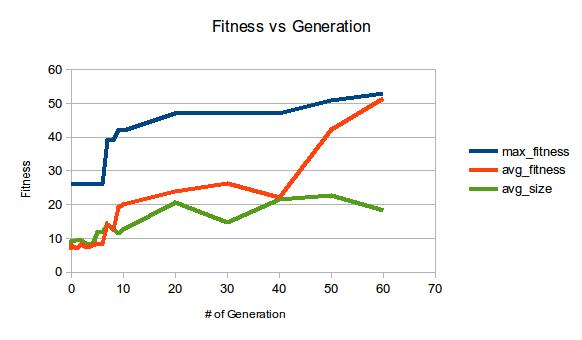
\includegraphics[width=.9\linewidth]{./fig1.jpg}
\caption{Average and best fitness for the symbolic problem. Best fitness has the perfect trend, but average fitness has several peaks due to the offspring outliers resulted from parent crossover and node mutation.}
\end{figure}
Figure 1 indicates that the crossover and node mutation works pretty well in that aspect that the best individual fitness from the population reduced down smoothly. 
From the above figure 1 we can also see that the average fitness has several peaks, that was due to the offspring outliers when two parent from previous generation crossover and node mutated. If I apply some tricks to filter out these outliers, and then calculate the population average, it should be able to get smoothly down average fitness as well.
\subsection{Applying best function on test points}
\label{sec-2-2}
\begin{lstlisting}[language=c++]
/ @ @ X . / / / / / / . . . . . . . / . / / / / / / / / / . . . 
/ / / @ / / . . / / / / . . . . . / / . . / . / / / / / / . . . 
. / / @ / / / / / . . / . . . . . / / / / / . / / X @ @ / / . . 
. . / @ / / / / / / / / . . . . . . / / / / / / @ . . / . @ / . 
. . . @ . / / / / / / / / . . . . . / / . . / / @ / / / . X / . 
. . / @ X X @ . @ @ @ @ @ / . . . . / / / @ @ . . / / / / / / . 
. . / / / / / . . / . / @ / / . . . . . / / / / / / . . / @ / / 
. . / / / / / / / / . . @ . / / . . . . X / / / / / / / / . . / 
. . / / / . . / / / / / @ . . / . . . . X . / / / / / / / / / / 
/ . . / / / / / . . / / @ / / / . . . . X . . / . / / / / @ / / 
/ / . . . / / / / / / . . / / / / . . . X . / / . . / . / / / / 
/ / / . . / / / / / / / @ / . . / . . . . . / / / / / . / / . / 
/ . / / . . / / / / / / / / / / / . . . . . . . / / / / / @ . . 
/ . . / . . / / / . / / @ / / / / / . . X . . / / . . / / / / / 
/ / / / . . . / / . . / X / / / / / / . X . . / / / @ @ X . / / 
. / / / / . . / / / / / . . / . / @ / / . . . X . / / / / / / . 
/ / . . / . . . / / / / / / / . . / . / / . . . . . / / / / / / 
/ / / / / . . . / / . . @ / / / / / . . / . . . . . . / / / / / 
/ / / / / / . . / / / / @ . . / @ / / / / . . . X . . . / / / / 
. / / / / / / . . . / / @ / / / X . / / / / . . . . . @ / . . / 
. . / . / / / / . . . / @ / / / @ / / . . / . . . . . / / / / / 
/ / / . . / . / / . . . @ / / / @ / / / / / . . . . . . . / / / 
/ / / / / / . . / . . . X / . / / / / / / / / . . . X . / / / . 
/ . . / / / / / / . . . @ / . . / . / / / / / @ . . . . / / / / 
/ / / @ X . / @ @ @ X X / / / / @ . . / . / / / / . . . . / / / 
/ @ / / / / / . . / . . . . / / @ / / / . . / . / / . . . . / / 
/ @ / / / / / / / / . . . / / . X / / / / / / . . / . . . . . . 
. @ . / / / / / / @ X X X @ @ / / / . . / / / / / / . . . . . . 
/ @ . . / . / @ / / . . . . . / / / / / / . . / / / / . . . . . 
/ / / / / . . @ . / / . . . . . / / / / / / / / . . / . . . . . 
. . @ @ @ @ / / . . / . . . . . . / / / / / / / / / / . . . . . 
\end{lstlisting}

As can be seen from above table, it is a working algorithm, or in other words, code set, but still it has some ditance away from the expected one. Recall the algorithm that I have used, it was the crossover step that I have restricted the crossover node too restricted. Except the 90/10 non-terminal terminal rule, I have also restricted the crossover to be non-terminal to non-terminal swap, or terminal to terminal swap, but I should have allow non-terminal to terminal or terminal to non-terminal as well. 
And as mentioned earlier, I didn't bother to apply the isFoodAhead function, which means if I have controlled the forward node of the isFoodAhead non-terminal, the ant should be able to behave smarter, and potentially being able to pick up more food, getting better fitness.
\section{Conclusions}
\label{sec-3}

In order be able to do genetic programming, we need certain data structures that would allow us be able to swap the evoluationary algorithms data in the middle functionally as if we have swapped programs. Like this project, we used the tree structure. As far as we understand the Genetic Programming theory and C++ pointer, the project turned out to be not that hard. And so far, it works pretty well. 
And compared with project 2, I included an static ant in the node object so that the static ant is shared among all the node, subsequentially individuals and population. But in order to separate among individuals, the ant gets resetted to evaluate for each new individual.

But still, as can be easily seen from table 1, it works well, but there are quite some distance from the expert solutions. With deeper consideration of good-bad codes side-effects, and individual expression tree size control, together with better understanding of the relationship between the non-terminal and terminals having been applied and the behaviors the ant, by modifying and enforcing the isFoodAhead non-terminal's "forward" terminal node, and potentially including an isFood2StepsAhead, which looks ahead 2 steps away, potentially my static ant will still behaviors smarter and smarter. But it is good to see that the ant is smarter enough to evolve evolutionary genetic programming like, which means the algorithms in this project works.
\section{example results I got before bad$_{\text{alloc}}$}
\label{sec-4}

\begin{lstlisting}[language=c++]
[jenny@jenny-G50VT][~/docu/572/p]% a
. X X X . . . . . . . . . . . . . . . . . . . . . . . . . . . . 
. . . X . . . . . . . . . . . . . . . . . . . . . . . . . . . . 
. . . X . . . . . . . . . . . . . . . . . . . . . X X X . . . . 
. . . X . . . . . . . . . . . . . . . . . . . . X . . . . X . . 
. . . X . . . . . . . . . . . . . . . . . . . . X . . . . X . . 
. . . X X X X . X X X X X . . . . . . . . X X . . . . . . . . . 
. . . . . . . . . . . . X . . . . . . . . . . . . . . . . X . . 
. . . . . . . . . . . . X . . . . . . . X . . . . . . . . . . . 
. . . . . . . . . . . . X . . . . . . . X . . . . . . . . . . . 
. . . . . . . . . . . . X . . . . . . . X . . . . . . . . X . . 
. . . . . . . . . . . . . . . . . . . . X . . . . . . . . . . . 
. . . . . . . . . . . . X . . . . . . . . . . . . . . . . . . . 
. . . . . . . . . . . . X . . . . . . . . . . . . . . . . X . . 
. . . . . . . . . . . . X . . . . . . . X . . . . . . . . . . . 
. . . . . . . . . . . . X . . . . . . . X . . . . . X X X . . . 
. . . . . . . . . . . . . . . . . X . . . . . X . . . . . . . . 
. . . . . . . . . . . . . . . . . . . . . . . . . . . . . . . . 
. . . . . . . . . . . . X . . . . . . . . . . . . . . . . . . . 
. . . . . . . . . . . . X . . . X . . . . . . . X . . . . . . . 
. . . . . . . . . . . . X . . . X . . . . . . . . . . X . . . . 
. . . . . . . . . . . . X . . . X . . . . . . . . . . . . . . . 
. . . . . . . . . . . . X . . . X . . . . . . . . . . . . . . . 
. . . . . . . . . . . . X . . . . . . . . . . . . . X . . . . . 
. . . . . . . . . . . . X . . . . . . . . . . X . . . . . . . . 
. . . X X . . X X X X X . . . . X . . . . . . . . . . . . . . . 
. X . . . . . . . . . . . . . . X . . . . . . . . . . . . . . . 
. X . . . . . . . . . . . . . . X . . . . . . . . . . . . . . . 
. X . . . . . . X X X X X X X . . . . . . . . . . . . . . . . . 
. X . . . . . X . . . . . . . . . . . . . . . . . . . . . . . . 
. . . . . . . X . . . . . . . . . . . . . . . . . . . . . . . . 
. . X X X X . . . . . . . . . . . . . . . . . . . . . . . . . . 
Population Information: 
min:26
avg:6.5
avgSize:7.16667
00       26      6.5    0        7.16667
0        26      8      3        9.16667
1        26      7      3        9.5
2        26      8.16667        3        9.5
3        26      7.33333        26       8.16667
4        26      7.83333        26       8.16667
5        26      8.5    26       11.8333
6        26      8.33333        26       11.6667
7        39      14.3333        3        14
8        39      12.5   26       12.6667
9        42      19.1667        26       11.3333
10       42      20     0        12.5
20       47      24     39       20.5
30       47      26.1667        2        14.6667
40       47      22     11       21.6667
50       51      42.1667        51       22.8333
60       53      51.3333        51       18.1667
got here popu reachBest
\end{lstlisting}
\section{A expression tree I have got}
\label{sec-5}
This fitness function is used for the test points plot, because this is the best tree that I have been able to save the expression tree results. Previous ones, like some function fitness can reach down to 35.9268, but I lost tract of the individuals when I got bad$_{\text{alloc}}$. 
\begin{lstlisting}[language=c++]
popu[1]:  Size: 31 Fitness: 64
P3->1
        P2->0
                R->4
                L->3
        P3->1
                P2->0
                        R->4
                        L->3
                P2->0
                        R->4
                        L->3
                P3->1
                        P2->0
                                R->4
                                F->5
                        P2->0
                                R->4
                                L->3
                        iFA->2
                                L->3
                                F->5
        P3->1
                P2->0
                        R->4
                        F->5
                P2->0
                        R->4
                        L->3
                iFA->2
                        L->3
                        F->5
\end{lstlisting}
% Emacs 24.3.50.1 (Org mode 8.2.5h)
\end{document}